\documentclass{article}
\usepackage{graphicx}
\graphicspath{ {./images} }
\usepackage{float}
\title{Capstone Project Report}
\date{}
\author{Marcel Stolin \\ marcelstolin@gmail.com}

\begin{document}

\maketitle

%############
\section{Definition} \label{s_definition}

\subsection{Project Overview} \label{su_project_overview}
Image classification is an active research field in multimedia. Applications of image classification are widely used in security, healthcare, entertainment and many more to face real world problems.\newline
The goal of this project is to develop an image classifier to predict dog breeds and it is mainly created for entertainment purposes. However, serious research projects about animal classification exists. For example Trnovszky, Kamencay, Orjesek, Benco and Sykora published a paper where they created a Convolutional Neural Network (CNN) to propose the animal species from an images of an animal \cite{animal_rec}.\newline
This projects is also one of the options, given by Udacity, for a capstone project. It comes with a predefined problem statement and a Jupyter Notebook to complete. Udacity also provides the data of dog images and human images. The dataset for dog images is a custom dataset from Udacity. The images of human faces come from the LFW (Labeled Face in the Wild) \cite{lfw} dataset from the University of Massachusetts.

\subsection{Problem Statement} \label{su_problem_statement}
As mentioned in section \ref{su_project_overview} this project comes with a predefined problem statement and a Jupyter Notebook. The main goal is to create a CNN to predict a dog breed from a given image. If the image only shows a human, then the algorithm will detect the human and return the dog breed for the human face. To achieve the project goal, a CNN has to be made from scratch or a pretrained model has to be used. To create a CNN from scratch and compare the performance to a pretrained model is a mandatory task in this project.\newline

According to this information and to the given Jupyter Notebook, the project can be cur down to the following ordered list of problems:
\begin{enumerate}
	\item Create a human face detector
	\item Create a dog detector
	\item Create a CNN to predict the dog breed
	\item Create an algorithm, which will return the predicted dog breed for the image
\end{enumerate}
The listed points are just a simple overview for the whole project. The given data also needs to be imported and processed, which is described in detail in section \ref{su_preprocessing}.\newline

The algorithm comes with it own requirements:
\begin{enumerate}
	\item The image shows a dog \(\Rightarrow\) Return the predicted dog breed
	\item The image shows a human \(\Rightarrow\)  Return the predicted dog breed with a different text
	\item The image shows neither man nor human \(\Rightarrow\)  Print an error message
\end{enumerate}

\subsection{Metrics} \label{su_metrics}
To evaluate a classification model, it is common to use the Accuracy, Precision, Recall and F1-Score metric. A Confusion Matrix can be used to visualize the results of a classifier.\newline

\paragraph{Confusion Matrix} The Confusion Matrix makes it it easy to see if a model confuses a class. All above mentioned metrics are based on a Confusion Matrix.
\begin{figure}[h]
    \centering
    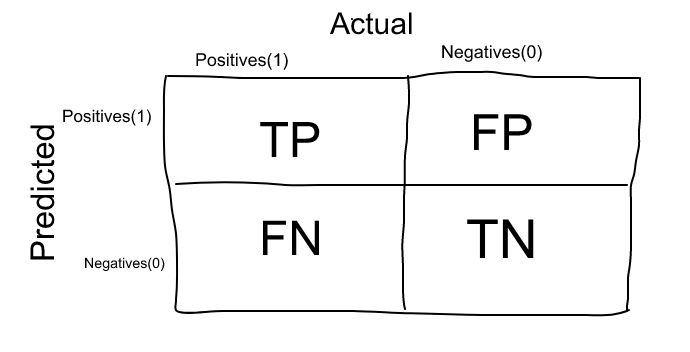
\includegraphics[scale=0.35]{./images/confusion_matrix}
    \caption{Confusion Matrix \cite{metrics}.}
    \label{fig:confusion_matrix}
\end{figure}
\begin{itemize}
    \item \textbf{True Positives (TP)} are cases when the actual class and the predicted are True (1)
    \item \textbf{False Positives (FP)} are cases when the actual class is False (0) and the predicted is True (1)
    \item \textbf{True Negatives (TN)} are cases when the actual class and the predicted class are False (True)
    \item \textbf{False Negatives (FN)} are cases when the actual class  is True (1) and the predicted is False (0)
\end{itemize}

\paragraph{Accuracy} Accuracy is the number of correct predictions made over all predictions.
\begin{equation}
Accuracy = \frac{TP + TN}{TP + FP + FN + TN}
\end{equation}

\paragraph{Precision} Precision is measure which tells us, what proportion of predicted positives are truly positives.
\begin{equation}
Precision = \frac{TP}{TP + FP}
\end{equation}

\paragraph{Recall} The recall metric tells us, what proportion of actual positives are correctly classified.
\begin{equation}
Recall = \frac{TP}{TP + FN}
\end{equation}

\paragraph{F1-Score} The F1-Score is the harmonic mean of precision and recall.
\begin{equation}
F1 Score = 2 * Precision * \frac{Recall}{Precision + Recall}
\end{equation}
%############

%############
\section{Analysis} \label{s_analysis}

\subsection{Data Exploration} \label{su_data_expl}
The dog images dataset has already been split into test, train, and valid sets. In total the dataset contains 8351 image files of 133 unique dog breeds. The images of the Udacity dog dataset have different dimensions, therefore the images have to be resized, which is described in detail in section \ref{su_preprocessing}. The LFW dataset contains 13234 images of 5749 unique individuals. Images in the LFW dataset have a dimension of 250x250 pixels.\newpage

\begin{figure}[h]
    \centering
    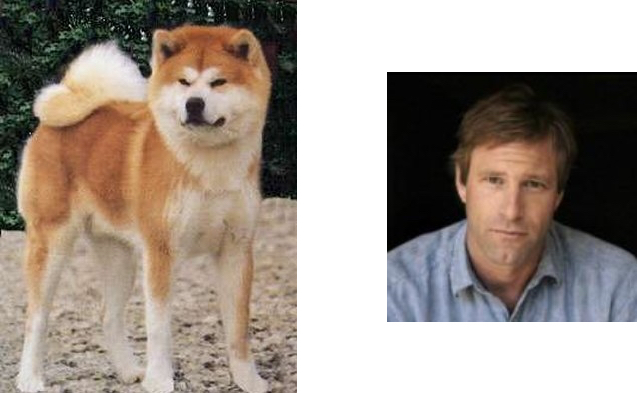
\includegraphics[scale=0.35]{./images/dataset_example}
    \caption{Example images from the datasets. The first images shows the Akita breed, the second image shows the actor Aaron Eckhart.}
    \label{fig:dataset_example}
\end{figure}
\newpage

\subsection{Exploratory Visualization} \label{su_expl_vis}
\begin{figure}[H]
    \centering
    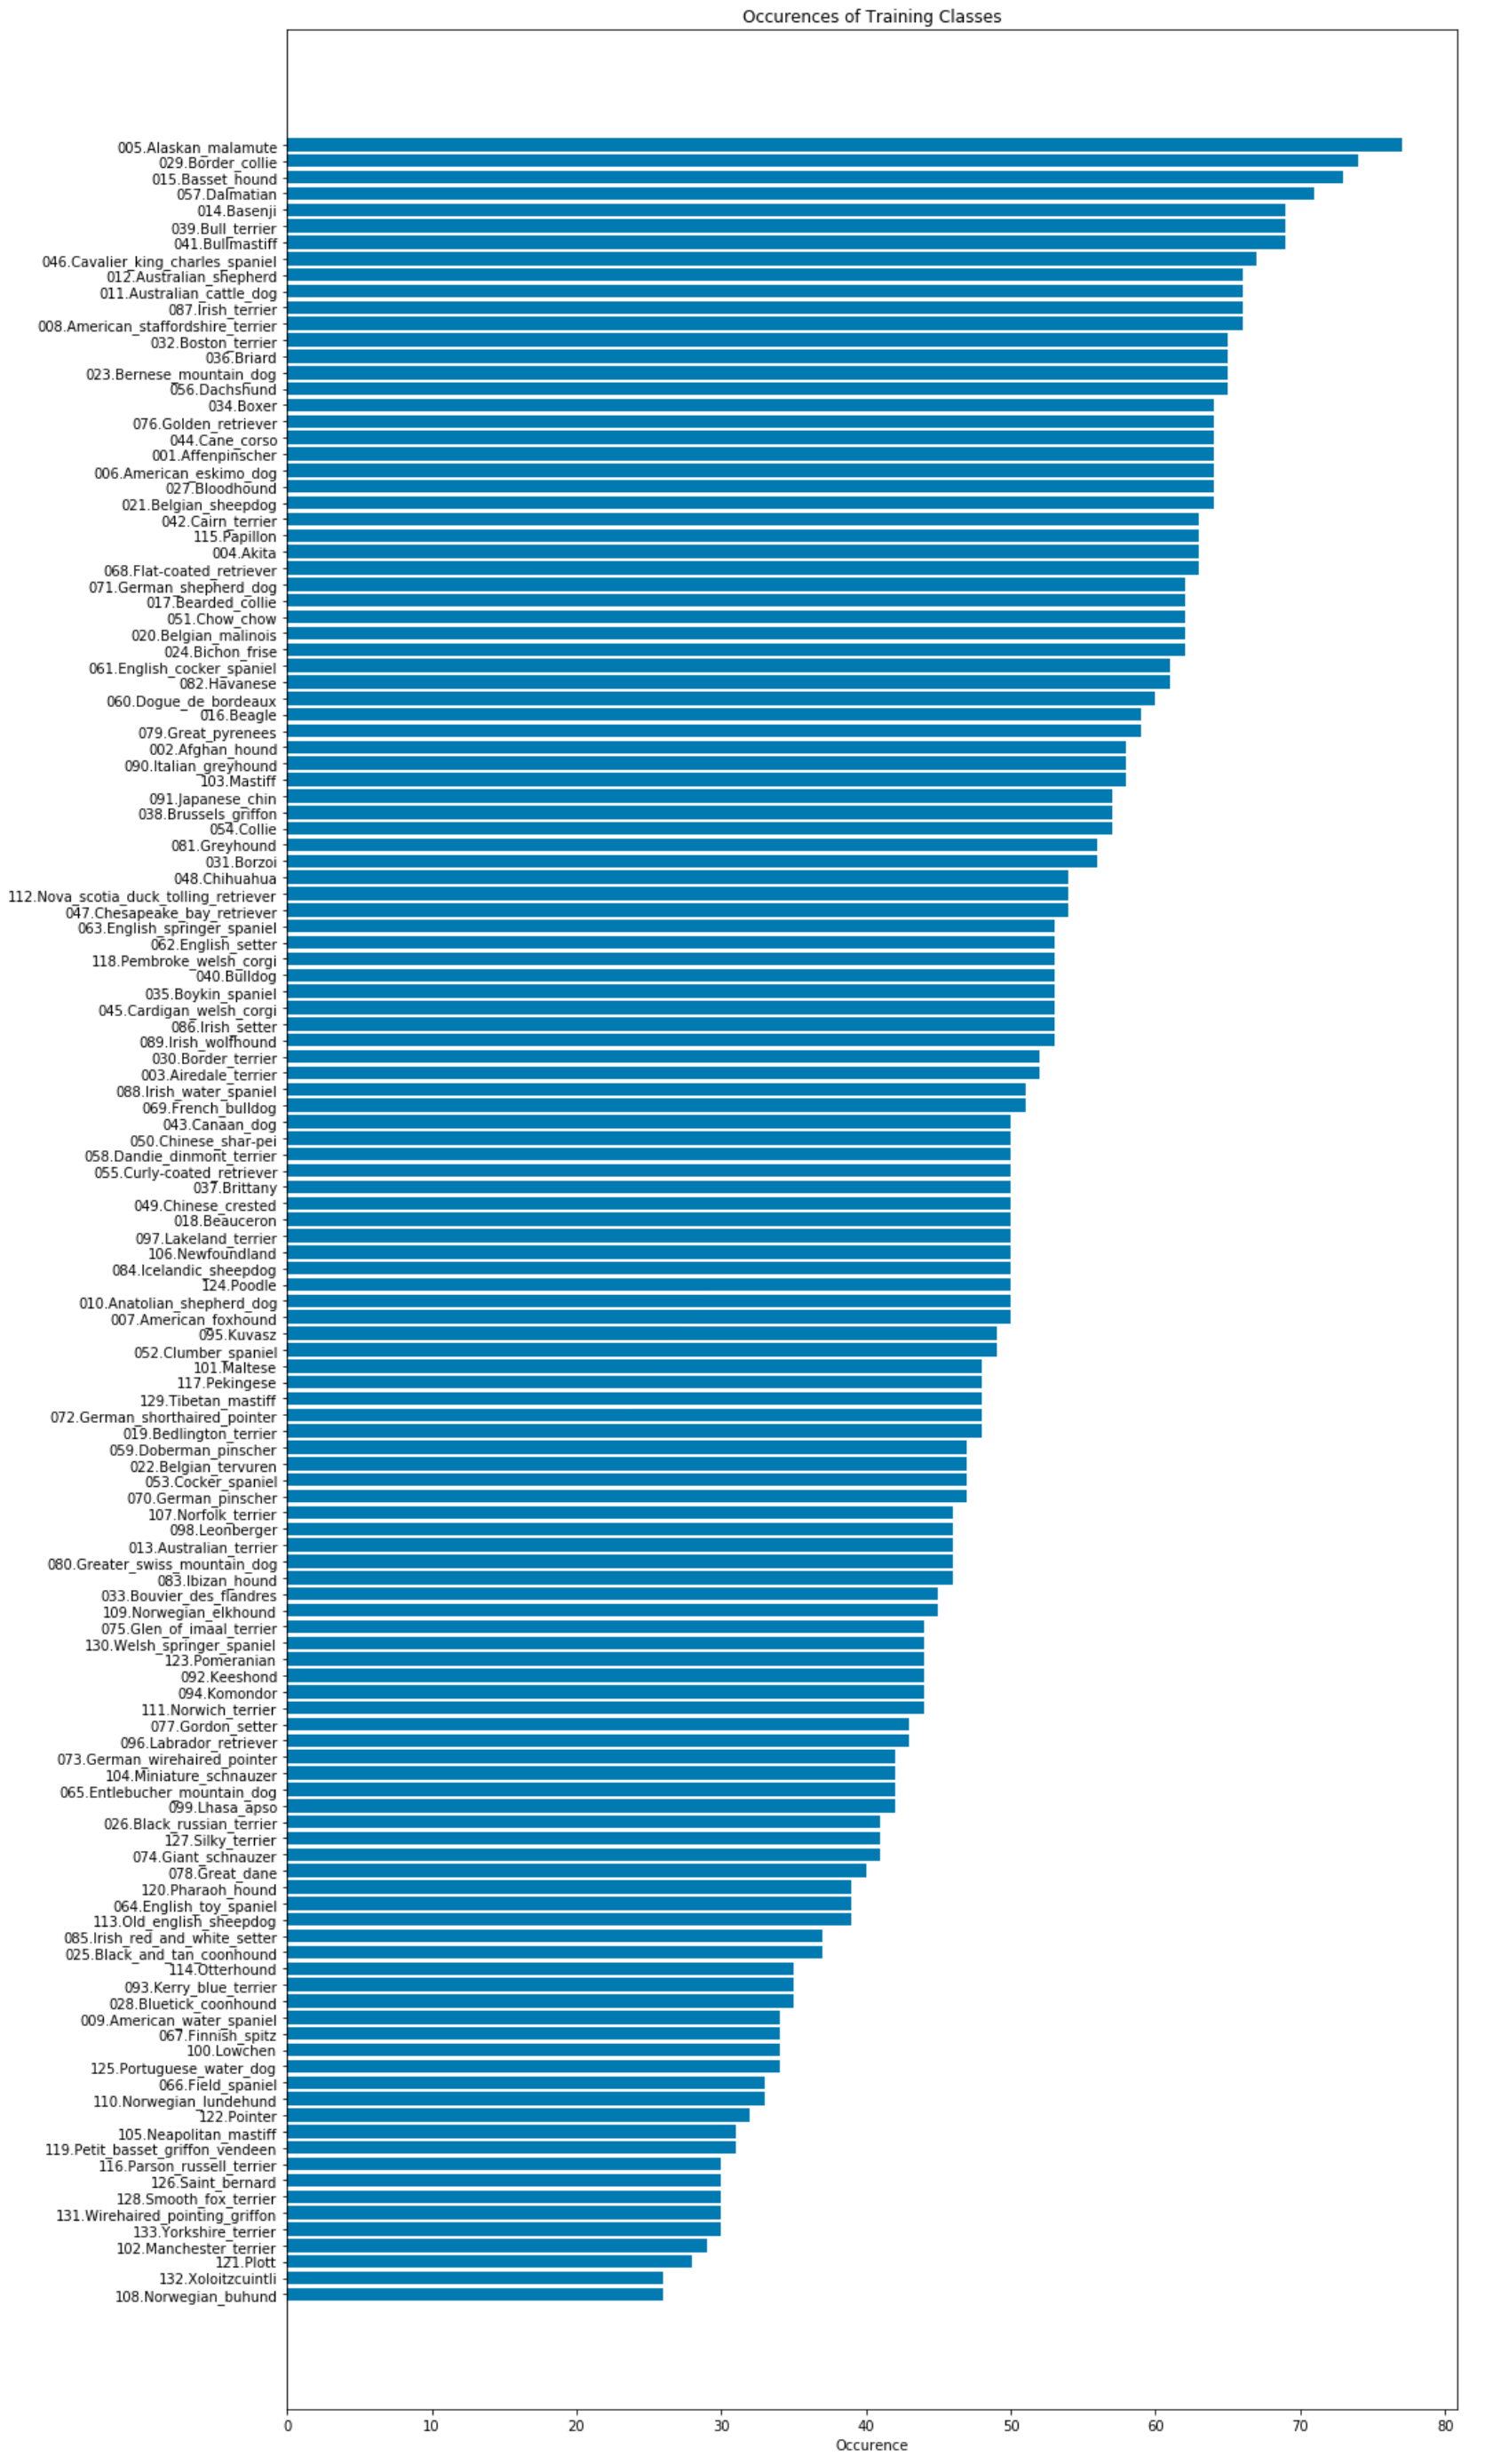
\includegraphics[scale=0.35]{./images/dog_breed_occurence}
    \caption{Visualization of dog breed occurences in the train dataset.}
    \label{fig:breed_occurence}
\end{figure}
Figure \ref{fig:breed_occurence} shows the occurences of each individual dog breed in the train dataset. As the bar shows, the breeds are not evenly distributed. Therefore the CNNs of this project, will predict dog breeds with a higher occurence (e.g. Alaskan Malamute), better than breeds with a lower occurence (e.g. Norwegian Buhund).

\subsection{Algorithms and Techniques} \label{su_alg_and_techn}
\paragraph{Face Detection} One part of the problem is to detect humans. Therefore a detector for human faces is needed. OpenCV provides the Haar Cascade classifier \cite{haar_cascade}. The classifier is trained from images with an machine learning approach based on a cascade function, to detect objects in images \cite{opencv}. OpenVC provides three different pretrained models to detect human faces: \textsf{FrontalFaceAlt}, \textsf{FrontalFaceAlt2}, \textsf{FrontalFaceDefault}. The comparison result showed, that \textsf{FrontalFaceAlt} is the best pretrained model for our use case. The model has an accuracy of 100\% for human faces.
\begin{figure}[h]
    \centering
    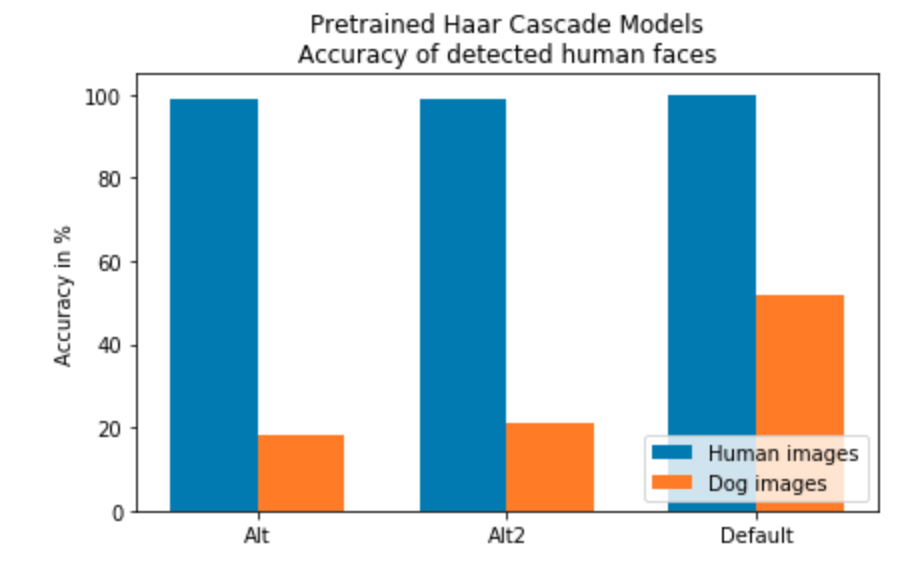
\includegraphics[scale=0.45]{./images/haar_cascades_results}
    \caption{Accuracy comparison of all three Haar cascade models.}
    \label{fig:haar_cascace_comp}
\end{figure}

\paragraph{Dog Detection} VGG-16 \cite{vgg} is a useful pretrained network to detect dogs. The VGG-16 network is recommended by the creators of the provided notebook. It is also possible to use other pretrained networks like Inception-v3 or ResNet-50 \cite{resnet}. I decided to focus on VGG-16 for the dog detection, because in Transfer Learning, the ResNet-50 network will be used anyway.
\begin{figure}[h]
    \centering
    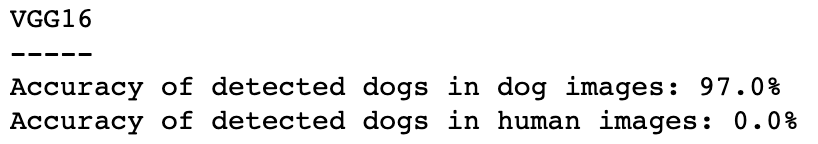
\includegraphics[scale=0.45]{./images/vgg16_dog_detector}
    \caption{Output of the VGG-16 model accuracy on the training datasets.}
    \label{fig:dog_detection_acc}
\end{figure}

\paragraph{Dog Classifier} This project has two mandatory tasks: Create a CNN from scratch and create a CNN using Transfer Learning. To create a CNN from scratch, the framework provided by the notebook is PyTorch. PyTorch is a machine learning library developed by facebook \cite{pytorch}.\newline
For Transfer Learning I have decided to use the ResNet-50 pretrained network. The ResNet-50 network is trained with 152 layers on the ImageNet dataset and has won the 1st price on the ILSVRC 2015 classification task \cite{resnet}. Therefore, the ResNet-50 is the best fit for the problem of this project.

\subsection{Benchmark} \label{su_benchmark}
The benchmark requirements of this project are: The CNN made from scratch has to have an accuracy greater than 10\% and the Transfer Learning CNN has to have an accuracy greater than 60\%. The requirements are mandatory tasks from Udacity.\newline
There are no requirements about the dog detector or the human face detector. I have decided that an accuracy of at least 90\% has to be reached for these models.

%############
\section{Methodology} \label{s_methodology}

\subsection{Data Preprocessing} \label{su_preprocessing}
The ResNet-50 network is trained with images of a 224x224 dimension. Therefore I decided to use that image size for the network I have to create from scratch. I will also use the same values for image normalization parameters like torchvision. The torchvision normalization parameters are:
\begin{itemize}
    \item \textbf{mean:} [0.485, 0.456, 0.406]
    \item \textbf{std:} [0.229, 0.224, 0.225]
\end{itemize}
According to these parameters, all input images will be preprocessed like the following:
\begin{enumerate}
	\item Resize to 224x224 with center crop
	\item Normalize with torchvision mean/std values
\end{enumerate}

The training data will be augmented, because it will increase the diversity of the test data, without adding new images and prevents overfitting. I decided to augment the images with a random horizontal flip and random rotation. Only horizontal flipping is activated, because dogs cant be upside down. The training images will be preprocessed like the following:
\begin{enumerate}
	\item Randomly resize the image to 224x224 with center crop
	\item Random horizontal flip
	\item Random rotation of 10 Degrees
	\item Normalize with torchvision mean/std values
\end{enumerate}

\subsection{Implementation} \label{su_implementation}
\paragraph{Split the Dataset} The first task  was to split the datasets into train, valid and test data. The DataLoader class from PyTorch is a good solution to handle this case. As mentioned in section \ref{su_data_expl}, the dataset has already been split into train, valid and test, therefore it was easy to create three custom DataLoader and load the specific files. How the images get preprocessed is explained in section \ref{su_preprocessing}.\newline

\paragraph{Create a CNN from scratch} The second task was to create a CNN from scratch. To accomplish that, the notebook provides the machine learning library PyTorch to handle this task.\newline
The CNN has three convolutional layers, the first two layers have a stride of 2 to downsize the input size by two. After each convolutional layer, the output will be normalized by a batch normalization layer. After that, the ReLU activation function will be applied to the output. A max. pooling layer will downsize the output of each convolutional layer by two, after batch normalization and ReLU activation. To prevent overfitting the CNN has a dropout layer, the probability that an element will be zero-ed is 0.3. To create the output of the CNN, two fully connected linear layers will produce the 133-dim output.\newline
For training, the Cross Entropy loss function and the Stochastic Gradient Descent (SGD) criterion have been used.
\begin{figure}[h]
    \centering
    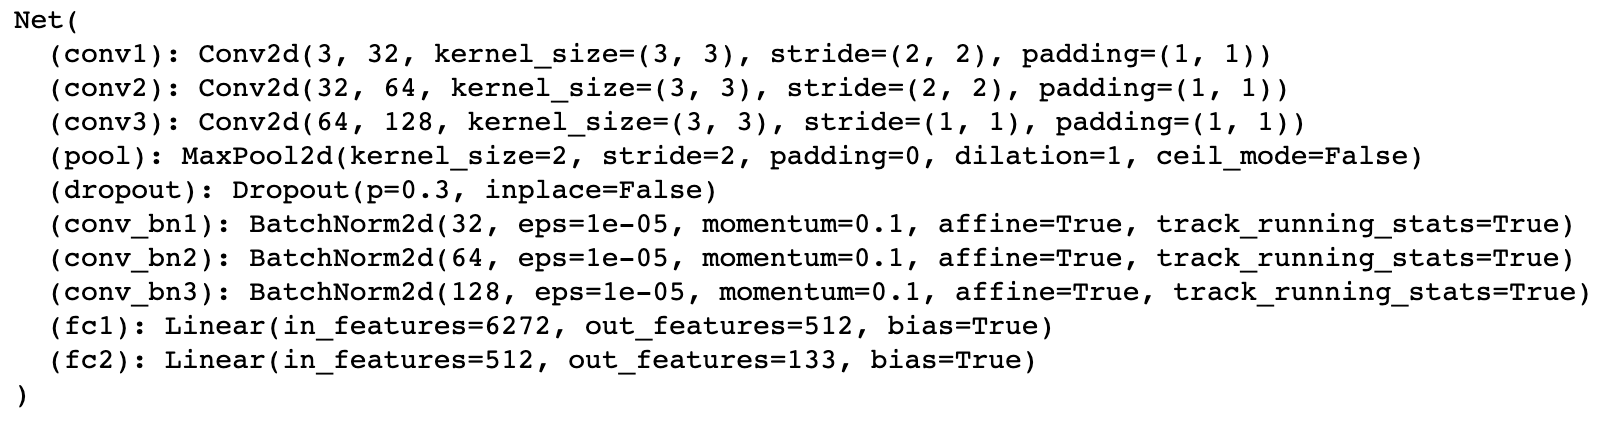
\includegraphics[scale=0.45]{./images/model_scratch_architecture}
    \caption{CNN architecture.}
    \label{fig:scratch_network_architecture}
\end{figure}

\paragraph{Transfer learning CNN} For the transfer learning implementation I have decided to use the ResNet-50 network, as mentioned in section \ref{su_alg_and_techn}. ResNet-50 is a pretrained network, so no architecture has to be defined by myself. The only thing that was necessary to complete the task, was to train the network with our train dataset. For training, the same loss function and criterion have been used.

\subsection{Refinement} \label{su_refinement}
%To create a CNN from scratch I tried a couple architecture before I got the final architecture. First I started with five convolutional layers and no batch normalization layer. The accuracy of that architecture was about 20\%. After I did some research about image classification CNNs I came up with the architecture explained in \ref{su_implementation}.\newline

To come up with a good number of epochs, I updated the train function to save and return a history of the loss and validation accuracy metric. At first, I started to train the CNN with 50 epochs. The visualization makes clear, that after the 40th epoch, no significant improvement has been made. The validation accuracy of the model will go up and down in range of 0.25 and 0.28. Also the validation loss stays between 2.9 and 3.0. Therefore I have decided to train the CNN with 40 epochs to prevent overfitting.
\begin{figure}[h]
    \centering
    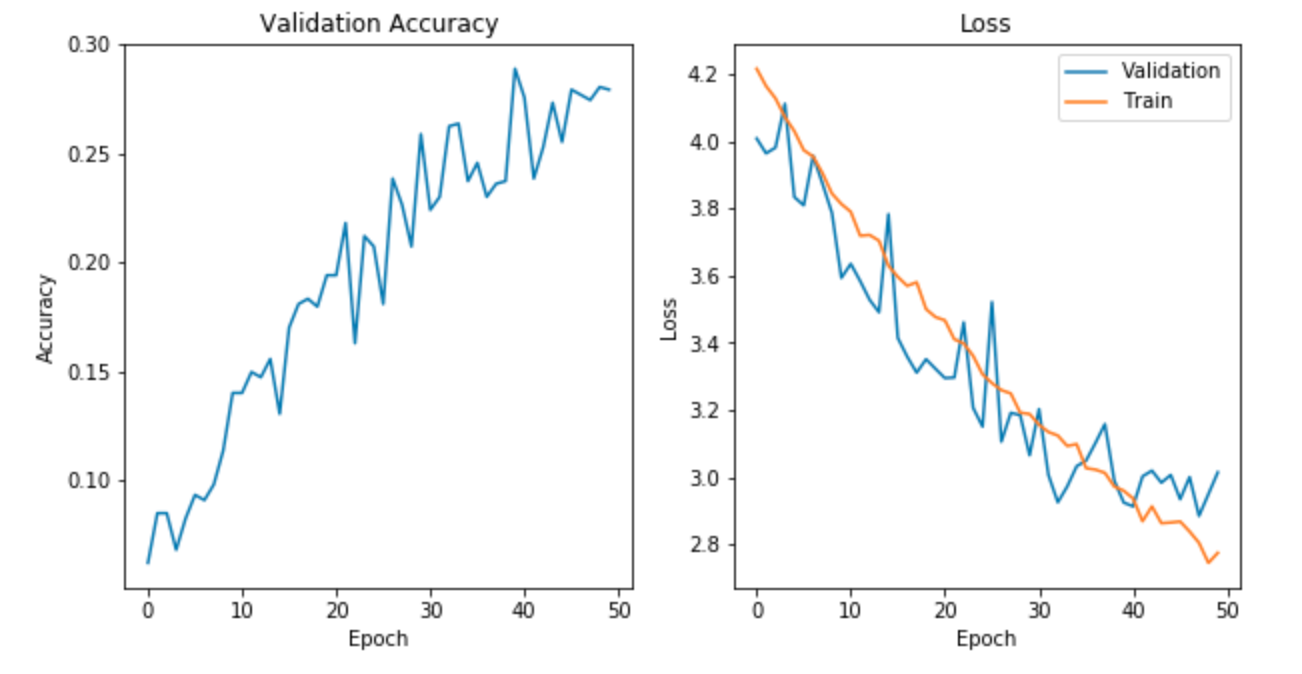
\includegraphics[scale=0.45]{./images/50_epochs}
    \caption{Accuracy and loss history of the CNN training.}
    \label{fig:cnn_train_metrics}
\end{figure}

%############
\section{Results} \label{s_results}

\subsection{Model Evaluation and Validation} \label{su_model_eval_val}
The model will be trained for several epochs. In each epoch the trained model gets validated against the validation dataset. The model with the lowest validation loss value will be saved. After training, the accuracy for the saved model gets determined. For testing the test dataset will be used.\newline
During this project, two networks will be trained, a network made from scratch and a pretrained network for transfer learning.

\subsubsection{Scratch CNN}
The network I had to create from scratch has a final accuracy of 27\% and a loss value of 2.96. Therefore the model hits the benchmark requirements.\newline
An accuracy of 27\% is not a good result for an image classification model. The classification report makes clear that the network is not able to detect 31 breeds out of 133. All of these 33 breeds have a precision, recall and F1-score value of 0. Because of these results, I decided to use a pretrained network for the transfer learning task.
\begin{figure}[h]
    \centering
    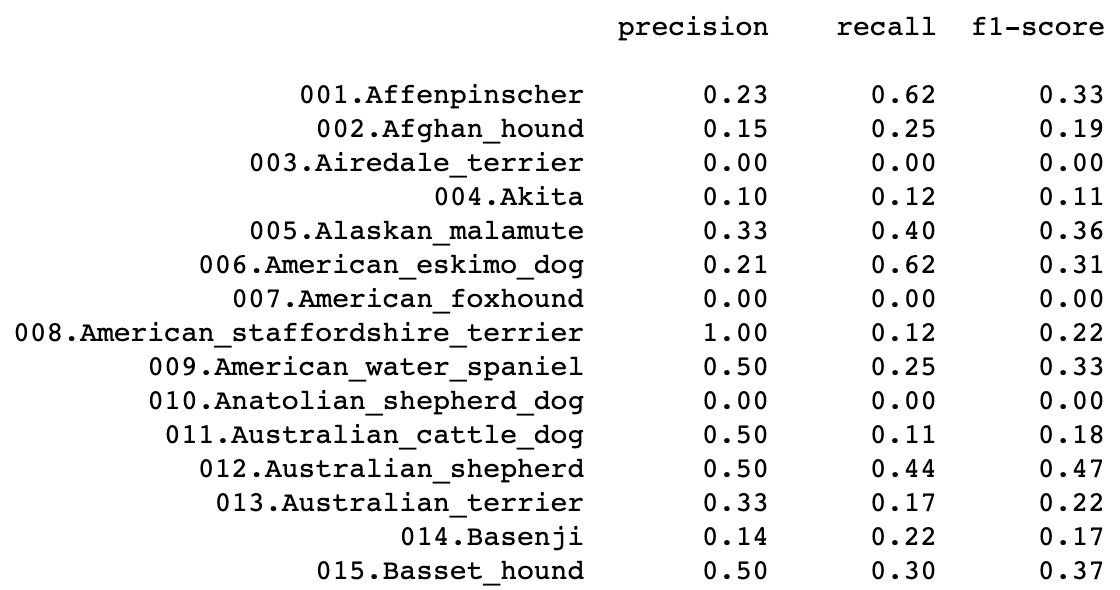
\includegraphics[scale=0.45]{./images/scratch_classification_report}
    \caption{Classification metrics results of the scratch CNN for the first fifteen dog breeds.}
    \label{fig:scratch_cnn_class_rep}
\end{figure}


\subsubsection{Transfer Learning Pretrained CNN}
For transfer learning I have decided to use the ResNet-50 network, this is described in section \ref{su_alg_and_techn}. The pretrained model has reached a test accuracy of 81\% and a test loss value of 1.02. Therefore the model reaches the benchmark requirements.\newline
The model shows significant improvements in the classification report. There is no breed with a precision, recall or F1-score value of 0.
\begin{figure}[h]
    \centering
    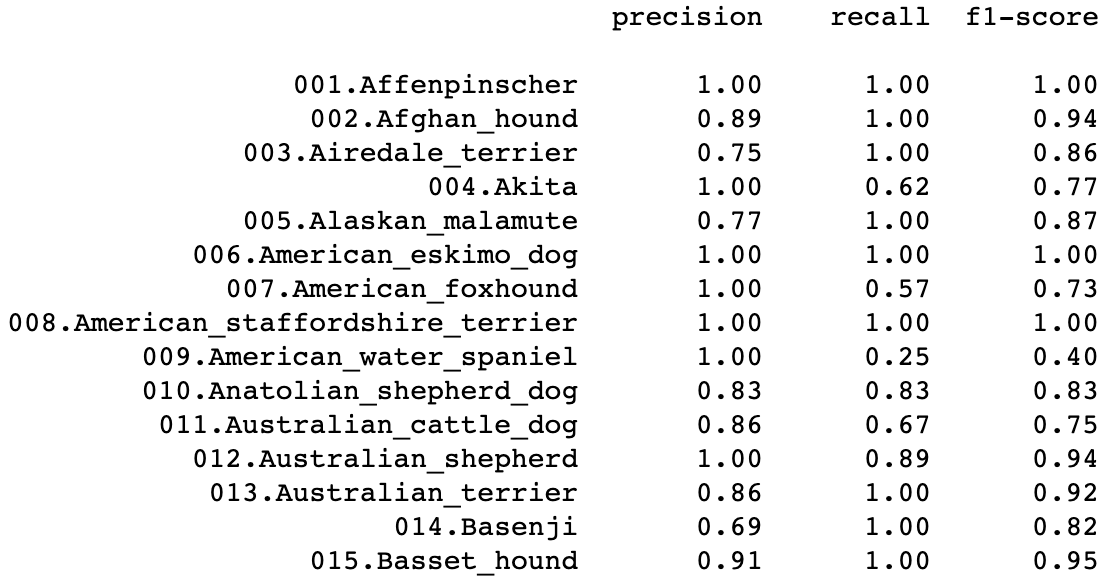
\includegraphics[scale=0.45]{./images/transfer_classification_report}
    \caption{Classification metrics results of the ResNet-50 for the first fifteen dog breeds.}
    \label{fig:scratch_cnn_class_rep}
\end{figure}

\subsection{Justification} \label{su_justification}
Both models exceeded the benchmarks and have therefore fulfill the requirements. The ResNet-50 network has an improvement of 54\% from the scratch CNN. The classification model makes clear, that the ResNet-50 outperformed the scratch CNN for each class by far.

\subsection{Algorithm} \label{su_algorithm}
The algorithm results are as expected. The algorithm is able to detect a dog breed, a human or something that is neither a dog nor a human.
\begin{figure}[H]
    \centering
    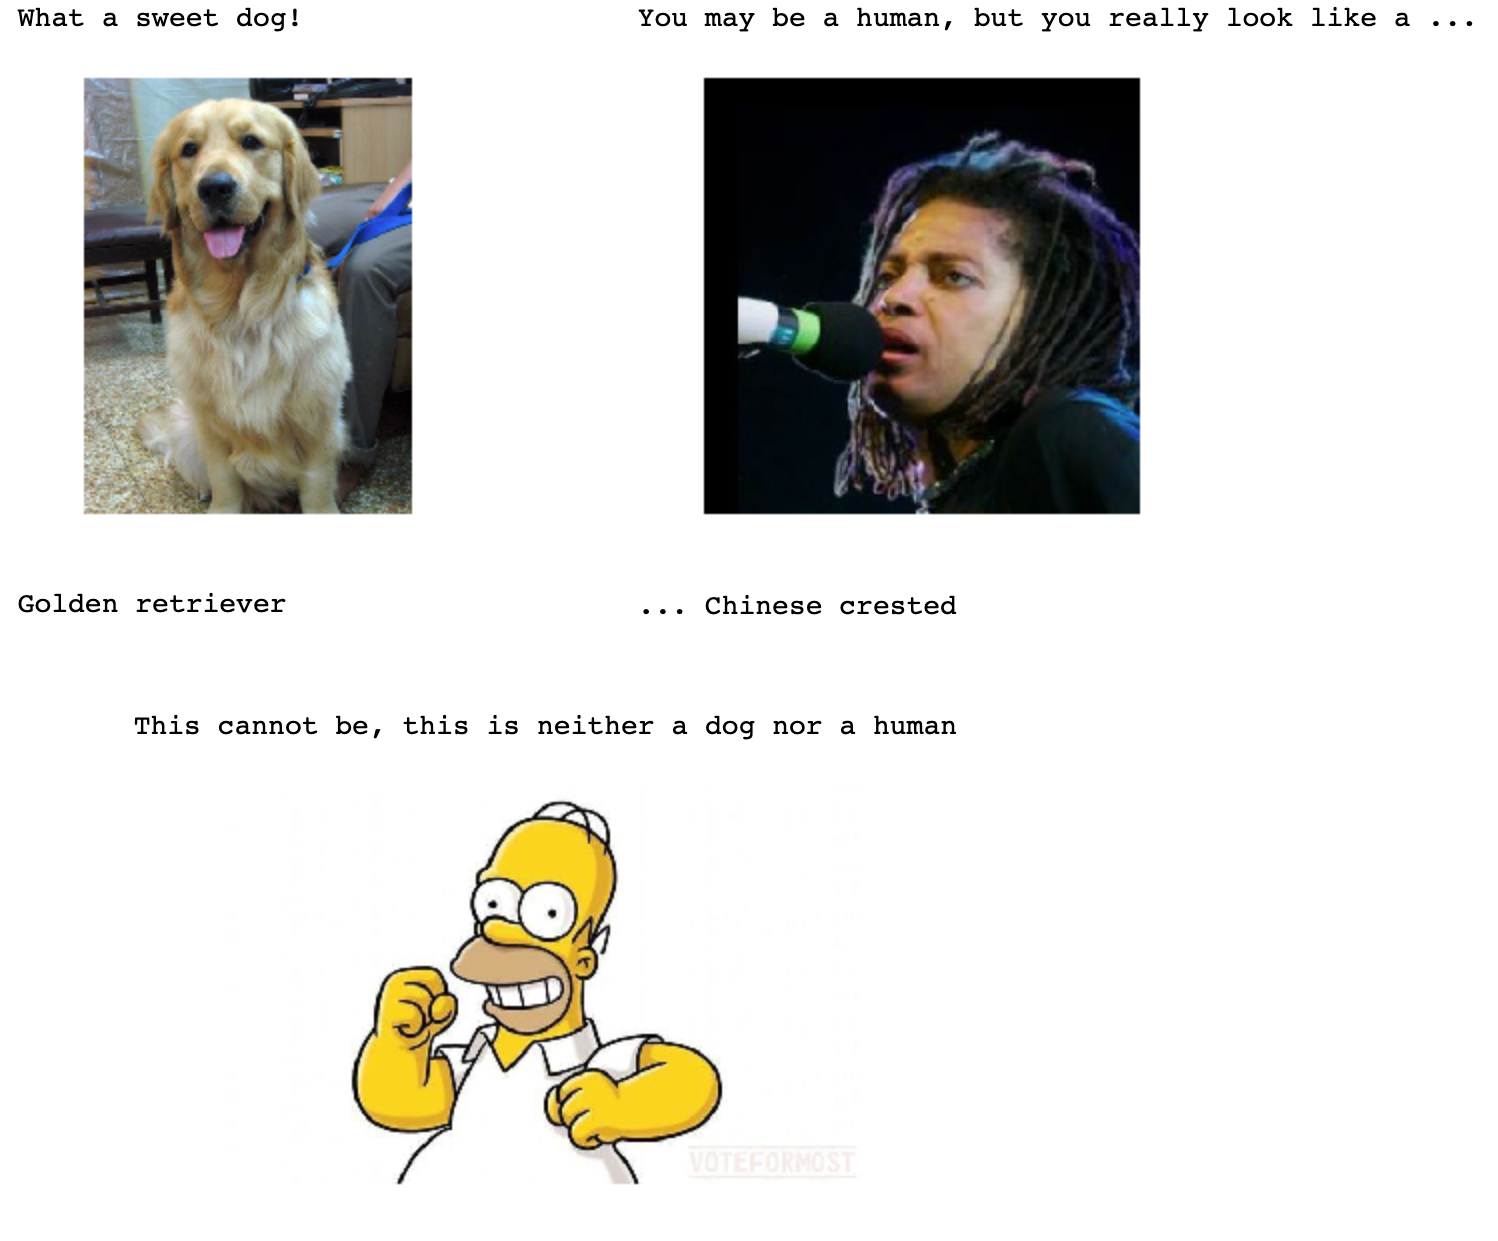
\includegraphics[scale=0.25]{./images/algorithm_result_true}
    \caption{Correct algorithms results.}
    \label{fig:algorithm_result_true}
\end{figure}

Since the model only reaches an accuracy of 81\% there are false predictions. In figure \ref{fig:algorithm_result_false} you can see two false predictions. The first dog is a West Highland White Terrier and the second dog is a black Labrador Retriever. The reason, why the model was not able to detect the West Highland White Terrier breed is, because the dog breed is not in the dataset. The model then returned the breed (Havanese) with the highest probability.
\begin{figure}[H]
    \centering
    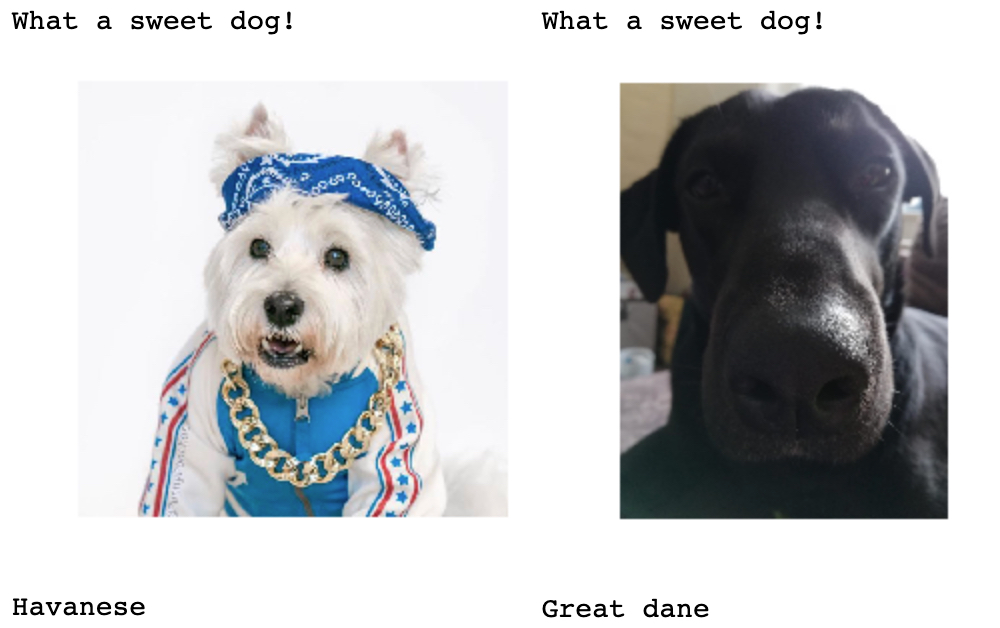
\includegraphics[scale=0.25]{./images/algorithm_result_false}
    \caption{False dog breed predictions.}
    \label{fig:algorithm_result_false}
\end{figure}

\paragraph{Improvements} In general the algorithm results are good. The algorithm fulfills all requirements and returns precise predictions. There are some points that can be improved.\newline
First, the algorithm is not able to predict more than one breed at a time. If the input is a group of at least two dogs, the algorithm will return only one prediction. It is also not clear which dog the algorithm will choose.\newline
Secondly, if the input is a couple of a dog and a human, the algorithm returns only the dog breed prediction. A better result would be the dog breed prediction and the dog breed prediction for the human.
\begin{figure}[H]
    \centering
    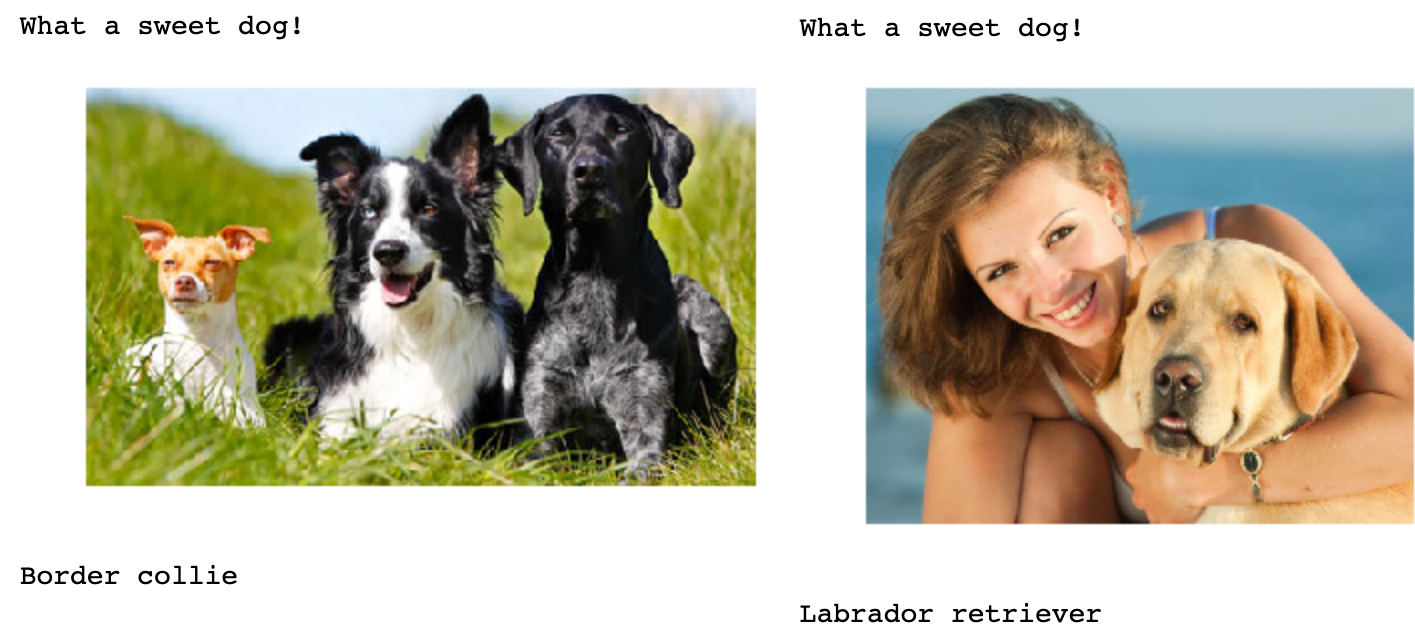
\includegraphics[scale=0.25]{./images/algorithm_improvements}
    \caption{Example outputs for improvements.}
    \label{fig:algorithm_improvements}
\end{figure}

%############
\bibliographystyle{plain}
\bibliography{references}
%############


\end{document}